%
% problemstellung.tex -- Beispiel-File für die Beschreibung des Problems
%
% (c) 2020 Prof Dr Andreas Müller, Hochschule Rapperswil
%


\section{Folgerungen
\label{laplace:section:folgerungen}}
Damit die Approximation von $\tilde{f}(t)$ möglichst genau $f(t)$ repräsentiert,
müssen die passenden Werte für $\lambda, \sigma $ und $\nu $ gefunden werden. 
Dies geschah in diesem Falle rein iterativ durch probieren.

Insbesondere wurden folgende Funktionen ausgewertet $ F_{1}(s)=\frac{1}{1-s} $ und $F_{2}(s) = \frac{2}{s^{3}}$. 
Die Werte welche für die Auswertung verwendet wurden sind in der Tabelle~\ref{laplace:parametertabelle} abgebildet.

\begin{table}
\centering
\begin{tabular}[c]{c|c|c}
& $F_{1}(s)=\frac{1}{1-s}$ & $F_{2}(s) = \frac{2}{s^{3}}$ \\
\hline
Parameter & $\lambda=1.288$ & $\lambda=0.101$ \\
& $\sigma=1.000001$ & $\sigma=0.965$ \\
& $\nu=0.81$ & $\nu=0.098953$ \\
\end{tabular}
\caption{XXX Beschreibung der Tabelle XXX
\label{laplace:parametertabelle}}
\end{table}
Die Abbildungen \ref{laplace:fehlerf1} -- \ref{laplace:fehler2-5} zeigen die Verläufe der absoluten Fehler.

\begin{figure}
\centering
%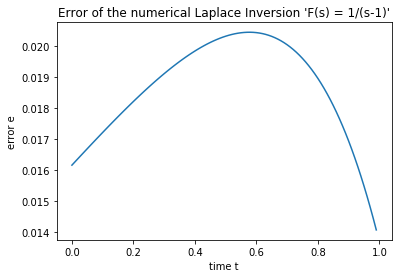
\includegraphics[width=8cm]{papers/laplace/Error_1divide_sminus1}
\caption{Fehler von $F_{1}(s)$
\label{laplace:fehlerf1}
}
\end{figure}

\begin{figure}
\centering
%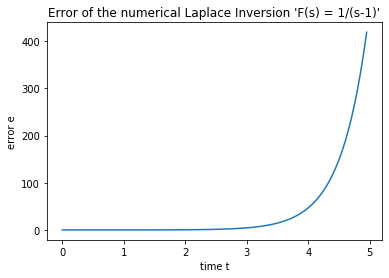
\includegraphics[width=8cm]{papers/laplace/Error_1divide_sminus1_bis_tgleich5}
\caption{Fehler von $F_{1}(s)$
\label{laplace:fehlerf1-5}
}
\end{figure}

\begin{figure}
\centering
%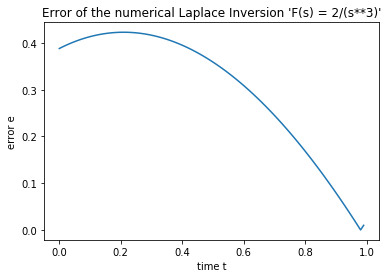
\includegraphics[width=8cm]{papers/laplace/Error_2divide_s_pow3}
\caption{Fehler von $F_{2}(s)$
\label{laplace:fehlerf2}
}
\end{figure}

\begin{figure}
\centering
%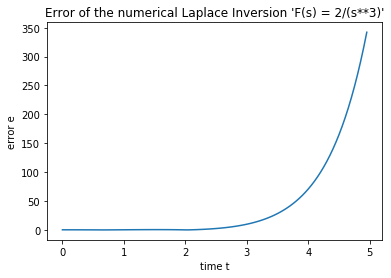
\includegraphics[width=8cm]{papers/laplace/Error_2divide_s_pow3_bis_tgleich5}
\caption{Fehler von $F_{2}(s)$
\label{laplace:fehlerf2-5}
}
\end{figure}


Es ist deutlich ersichtlich, dass der Fehler nur für ein gewisses Zeitintervall akzeptabel ist. Im Bereich wo der Fehler sich in einem tolerierbaren Bereich befindet, wurden die Parameter $\lambda, \sigma $ und $\nu $ für ein bestimmtes $t_{0}$ ermittelt. 
Diese Parameter sind für andere Zeitpunkt $t_{x}$ nicht mehr sinnvoll. 
Für den Zeitpunkt $t_{0}=1$ wurden die Fehler in der Grössenordnung $10^{-8}$ respektive $10^{-6}$ erreicht. 
Dies geschah mittels Erhöhung der Iterationszahl N.

\begin{center}
\begin{tabular}[c]{c|c|c}
& $F_{1}(s)$ & $F_{2}(s)$ \\
\hline
Parameter & $\lambda=1.288$ & $\lambda=0.101$ \\
 & $\sigma=1.000001$ & $\sigma=0.965$ \\
 & $\nu=0.81$ & $\nu=0.098953$ \\
\hline
$t_{0}$ & $1$ & $1$ \\
\hline
Fehler & $1.7076~*~10^{-08}$ & $1.8447~*~10^{-06}$ \\
\end{tabular}
\end{center}


